% !TeX root = RJwrapper.tex
\title{\pkg{casebase}: An Alternative Framework for Survival Analysis and Comparison of Event Rates}
\author{by Sahir Rai Bhatnagar*, Maxime Turgeon*, Jesse Islam, James A. Hanley, and Olli Saarela}

\maketitle

\abstract{%
In clinical studies of time-to-event data, a quantity of interest to the clinician is their patient's risk of an event. However, methods relying on time matching or risk-set sampling (including Cox regression) eliminate the baseline hazard from the estimating function. As a consequence, the focus has been on reporting hazard ratios instead of survival or cumulative incidence curves. Indeed, reporting patient risk or cumulative incidence requires a separate estimation of the baseline hazard. Using case-base sampling, Hanley \& Miettinen (2009) explained how parametric hazard functions can be estimated in continuous-time using logistic regression. Their approach naturally leads to estimates of the survival or risk function that are smooth-in-time. In this paper, we present the \CRANpkg{casebase} R package, a comprehensive and flexible toolkit for parametric survival analysis. We describe how the case-base framework can also be used in more complex settings: non-linear functions of time and non-proportional hazards, competing risks, and variable selection. Our package also includes an extensive array of visualization tools to complement the analysis. We illustrate all these features through three different case studies. * SRB and MT contributed equally to this work.
}

\hypertarget{introduction}{%
\section{Introduction}\label{introduction}}

The semiparametric Cox model has become the default approach to survival analysis
even though Cox himself later suggested he would prefer to model the hazard function
directly. In a 1994 interview with Professor Nancy Reid, Sir David Cox was asked
how he would model a set of censored survival data, to which he responded: ``I
think I would normally want to tackle problems parametrically \ldots{} and if you want
to do things like predict the outcome for a particular patient, it's much more
convenient to do that parametrically'' (Reid 1994). Indeed, the most
relevant quantity in a clinical setting is often the 5- or 10-year risk of
experiencing a certain event given the patient's particular profile.
However, the most reported metric from a Cox model is the (potentially
time-dependent) hazard ratio (HR). The covariate-conditional
survival curve is arguably a more important
summary measure to report than the HR. While stepwise survival curves can be
computed with the Cox model, they require a second step to separately estimate
the baseline hazard (Breslow 1972).

Several authors have since pursued fully parametric approaches that made the
fitting of smooth survival curves more transparent and intuitive through
generalized linear models. The key feature of these procedures is splitting the
time axis into discrete intervals. Whitehead (1980) showed the
equivalence between a Cox model and a Poisson regression with a parameter for
each event time; Carstensen (2019) provides an exposition of this
equivalence with a real data example and supporting R code for computing
standard errors. Arjas \& Haara (1987) and Efron (1988) treated each
patient-day as a Bernoulli random variable with probability equal to the
discrete hazard rate. A potential issue with these approaches is that the
number of time bins need to be chosen by the data analyst. On the one hand, a fine grouping
of times may result in few (or none) events per interval, which then leads
to instability in the Newton-Raphson procedure for estimation
(Kalbfleisch and Prentice 2011, vol. 360, sec. 4.8), and large long-format datasets.
On the other hand, a coarse grouping could potentially mask
nonlinear trends in the hazard function.

Rather than discretizing time, Hanley \& Miettinen (2009)
selected a discrete set of person-time coordinates (``person-moments'') in
continuous time from all observed follow-up experience constituting the
study base. By doing so, they obtained a likelihood expression for the hazard
function that is equivalent to that of logistic regression with an offset term.
More specifically, all person-moments when the event of interest
occurred are selected as the case series, complemented by a randomly sampled
base series of person-moments serving as controls. This approach allows
flexible modeling of the hazard function by including functions of time as covariates
(e.g.~using splines or generalized additive models). Furthermore, time-dependent
covariates can be modeled through interactions with time. In short, Hanley \&
Miettinen (2009) use the well-understood logistic regression
for directly modeling the hazard function, without requiring a discrete-time model.

In this article, we present the \CRANpkg{casebase} R package (Bhatnagar et al. 2021)
which implements and extends the Hanley \& Miettinen (2009) approach for
fitting fully parametric hazard models and covariate-conditional survival curves
using the familiar interface of the \texttt{glm} function. Our implementation
includes extensions to other models such as penalized
regression for variable selection and competing risk analysis. In addition,
we provide functions for exploratory data analysis and visualizing the estimated
quantities such as the hazard function, survival curve, and their standard errors.
The ultimate goal of our package is to make fitting flexible hazards accessible
to end users who favor reporting absolute risks and survival curves
over hazard ratios.

In what follows, we first recap some theoretical details on case-base sampling
and its use for estimating parametric hazard functions. We then give a short
review of existing R packages that implement comparable features to \pkg{casebase}.
Next, we provide some details about the implementation of case-base sampling in
our package, and we give a brief survey of its main functions. This is followed
by three case studies that illustrate the flexibility and capabilities of
\pkg{casebase}. We show how the same framework can be used for non-linear
functions of time and non-proportional hazards, competing risks, and variable
selection via penalized regression. Finally, we end the article with a
discussion of the results and of future directions.

\hypertarget{theory}{%
\section{Theoretical details}\label{theory}}

As discussed in Hanley \& Miettinen (2009), the key idea behind case-base sampling is to consider the entire study base as an infinite collection of \emph{person-moments}. These person-moments are indexed by both an individual in the study and a time point, and therefore each person-moment has a covariate profile and an outcome status (i.e.~whether the event happened) attached to it. By estimating the probability of an event occurring at a particular person-moment, we can extract information about hazards and survival.

Therefore, we start by assembling all person-moments at which the event occurred; this collection of person-moments is what Hanley \& Miettinen call the \emph{case series}. The incidence of the case series is dictated by the hazard function of interest. Next, we sample a finite number of person-moments (blinded to case moments); this second collection of person-moments is what Hanley \& Miettinen call the \emph{base series}. The sampling mechanism for the base series is left at the discretion of the user, but in practice we find that sampling uniformly from the study base provides both simplicity and good performance. This is the default sampling mechanism in the package.

\hypertarget{likelihood-and-estimating-function}{%
\subsection{Likelihood and estimating function}\label{likelihood-and-estimating-function}}

To describe the theoretical foundations of case-base sampling, we use the framework of counting processes. In what follows, we abuse notation slightly and omit any mention of \(\sigma\)-algebras. Instead, following Aalen \textit{et al} (2008), we use the placeholder ``past'' to denote the past history of the corresponding process. The reader interested in more details can refer to Saarela \& Arjas (2015) and Saarela (2016). First, let \(N_{i}(t) \in \{0, 1\}\) be counting processes corresponding to the event of interest for individual \(i=1, \ldots,n\). For simplicity, we will consider Type I censoring due to the end of follow-up at time \(\tau\) (the general case of independent censoring is treated in Saarela (2016)). We are interested in modeling the hazard functions \(\lambda_{i}(t)\) of the processes \(N_i(t)\), and which satisfy
\[\lambda_{i}(t)\,\textrm dt = E[\,\textrm dN_{i}(t)\mid \mathrm{past}].\] The processes \(N_i(t)\) count the person-moments from the \emph{case series}.

To complement the case series, we sample person-moments for the base series. To do so, we specify the base series sampling mechanism as non-homogeneous Poisson processes \(R_i(t) \in \{0, 1, 2, \ldots\}\); the person-moments where \(\,\textrm dR_i(t) = 1\) constitute the base series. We note that the same individual can contribute multiple person-moments to the base series. The process \(Q_{i}(t) = R_i(t) + N_{i}(t)\) then counts both the case and base series person-moments contributed by individual \(i\). As mentioned above, the processes \(R_i(t)\) are specified by the user via its intensity function \(\rho_i(t)\). The process \(Q_{i}(t)\) is characterized by \(E[\,\textrm dQ_{i}(t)\mid\mathrm{past}] = \lambda_{i}(t)\,\textrm dt + \rho_i(t)\,\textrm dt\).

If the hazard function \(\lambda_{i}(t; \theta)\) is parametrized in terms of \(\theta\), we can define an estimator \(\widehat{\theta}\) by maximization of the likelihood expression
\[L_0(\theta) = \prod_{i=1}^n \exp\left\{ -\int_0^{\min(t_i,\tau)} \lambda_i(t; \theta)\,\textrm dt \right\} \prod_{i=1}^{n} \prod_{t\in[0,\tau)} \lambda_{i}(t;\theta)^{\,\textrm dN_{i}(t)},\]
where \(\prod_{t\in[0,u)}\) represents a product integral from \(0\) to \(u\), and where \(t_i\) is the event time for individual \(i\). However, the integral over time makes the computation and maximization of \(L_0(\theta)\) challenging using standard software.

Case-base sampling allows us to avoid this integral. By conditioning on a sampled person-moment, we get individual partial likelihood contributions of the form
\[P(\,\textrm dN_{i}(t) \mid \,\textrm dQ_{i}(t) = 1,\mathrm{past}) \stackrel{\theta}{\propto} \frac{\lambda_{i}(t; \theta)^{\,\textrm dN_{i}(t)}}{\rho_i(t) + \lambda_{i}(t;\theta)}.\]
By using the symbol \(\stackrel{\theta}{\propto}\), we mean that both sides of the expression are equal up to multiplicative factors that do not depend on \(\theta\). Therefore, an estimating function for \(\theta\) can be composed of these contributions as:
\begin{equation}
L(\theta) = \prod_{i=1}^{n} \prod_{t\in[0,\tau)} \left(\frac{\lambda_{i}(t; \theta)^{\,\textrm dN_{i}(t)}}{\rho_i(t) + \lambda_{i}(t;\theta)}\right)^{\,\textrm dQ_i(t)}. \label{eq:lik-function}
\end{equation}
When a logarithmic link function is used for modeling the hazard function, the above expression is of a logistic regression form with an offset term \(\log(1/\rho_i(t))\). Note that the sampling units selected in the case-base sampling mechanism are person-moments, rather than individuals, and the parameters to be estimated are hazards or hazard ratios rather than odds or odds ratios. Generally, an individual can contribute more than one person-moment, and thus the terms in the product integral are not independent. Nonetheless, Saarela (2016) showed that the corresponding partial likelihood score function has mean zero at the true value \(\theta=\theta_0\), and that the resulting estimator \(\widehat{\theta}\) is asymptotically normally distributed.

In Hanley \& Miettinen (2009), the authors suggest sampling the base series \emph{uniformly} from the study base. In terms of Poisson processes, their sampling strategy corresponds to a time-homogeneous Poisson process with intensity equal to \(\rho_i(t) = b/B\), where \(b\) is the number of sampled base series \emph{person-moments}, and \(B\) is the total population-time for the study base (e.g.~the sum of all individual follow-up times). More complex examples are also possible; see for example Saarela \& Arjas (2015), where the intensity functions for the sampling mechanism are proportional to the cardiovascular disease event rate given by the Framingham score. Non-uniform sampling mechanisms can increase the efficiency of the resulting maximum partial likelihood estimators.

\hypertarget{variance-estimates}{%
\subsection{Variance estimates}\label{variance-estimates}}

The asymptotic normality of \(\widehat{\theta}\) gives us an efficient way to estimate the variance of various estimators derived from the hazard function. For example, to construct confidence bands around risk functions and survival functions, we can use the following procedure:

\begin{enumerate}
\def\labelenumi{\arabic{enumi}.}
\tightlist
\item
  Compute \(\widehat{\theta}\) and its variance-covariance matrix \(V(\widehat \theta)\) which is obtained as part of the logistic regression output.
\item
  Sample \(B\) times from a multivariate normal \(N\left(\widehat{\theta}, V(\widehat\theta)\right)\).
\item
  For each sample, compute the survival function using Equation \eqref{eq:surv} below.
\item
  Use the pointwise quantiles of these survival function estimates to construct a pointwise confidence band for the survival function of interest.
\end{enumerate}

This procedure is similar to parametric bootstrap (Efron and Tibshirani 1994, sec. 6.5), but it can be more accurately described as a form of approximate Bayesian computation. As such, the validity of the confidence bands relies on the Bernstein-von Mises theorem (Van der Vaart 2000, vol. 3, chap. 10).

\hypertarget{common-parametric-models}{%
\subsection{Common parametric models}\label{common-parametric-models}}

Here we show that certain named distributions such as exponential, Weibull or Gompertz can be fit using our framework, though we are not restricted to such models. Let \(g(t; X)\) be the linear predictor such that \(\log(\lambda(t;X)) = g(t; X)\). Different functions of \(t\) lead to different parametric hazard models. The simplest of these models is the one-parameter exponential distribution which is obtained by taking the hazard function to be constant over the range of \(t\):

\begin{equation}
\log(\lambda(t; X)) = \beta_0 + \beta_1 X. \label{eq:exp}
\end{equation}
In this model, the instantaneous failure rate is independent of \(t\).\footnote{The conditional chance of failure in a time interval of specified length is the same regardless of how long the individual has been in the study. This is also known as the \emph{memoryless property} (Kalbfleisch and Prentice 2011).}

The Gompertz hazard model is given by including a linear term for time:

\begin{equation}
\log(\lambda(t; X)) = \beta_0 + \beta_1 t + \beta_2 X. \label{eq:gomp}
\end{equation}

Use of \(\log(t)\) yields the Weibull hazard which allows for a power dependence of the hazard on time (Kalbfleisch and Prentice 2011):

\begin{equation}
\log(\lambda(t; X)) = \beta_0 + \beta_1 \log(t) + \beta_2 X. \label{eq:weibull}
\end{equation}

\hypertarget{competing-risk-analysis}{%
\subsection{Competing risk analysis}\label{competing-risk-analysis}}

Case-base sampling can also be used in the context of competing risk analysis. Assuming there are \(J\) competing events, we can show that each sampled person-moment's contribution to the partial likelihood is of the form

\[\frac{\lambda_j(t)^{\,\textrm dN_j(t)}}{\rho(t) + \sum_{j=1}^J\lambda_j(t)},\]
where \(N_j(t)\) is the counting process associated with the event of type \(j\) and \(\lambda_j(t)\) is the corresponding cause-specific hazard function. As may be expected, this functional form is similar to the terms appearing in the likelihood function for multinomial regression with an offset term.\footnote{Specifically, it corresponds to the following parametrization for a multinomial random variable \(Y\): \begin{align*} \log\left(\frac{P(Y=j \mid X)}{P(Y = J \mid X)}\right) = X^T\beta_j + log(1/\rho), \qquad j = 1,\ldots, J-1.\end{align*}}

\hypertarget{variable-selection}{%
\subsection{Variable selection}\label{variable-selection}}

To perform variable selection on the regression parameters \(\theta \in \mathbb{R}^p\) of the hazard function, we can add a penalty to the likelihood and optimise the following equation:
\begin{equation}
\min _{\theta \in \mathbb{R}^{p}}\,\,-\ell\left(\theta\right)+\sum_{j=1}^p w_j p_{\lambda,\alpha}(\theta_j) \label{eq:penest}
\end{equation}
where \(\ell\left(\theta\right) = \log L(\theta)\) is the log of the likelihood function given in \eqref{eq:lik-function}, \(p_{\lambda,\alpha}(\theta_j)\) is a penalty term controlled by the non-negative regularization parameters \(\lambda\) and \(\alpha\), and \(w_j\) is the penalty factor for the \(j\)th covariate. These penalty factors serve as a way of allowing parameters to be penalized differently. For example, we could set the penalty factor for time to be 0 to ensure it is always included in the selected model.

\hypertarget{comparison-with-existing-packages}{%
\section{Comparison with existing packages}\label{comparison-with-existing-packages}}

Survival analysis is an important branch of applied statistics and epidemiology. Accordingly, there is already a vast ecosystem of R packages implementing different methodologies. In this section, we describe how the functionalities of \CRANpkg{casebase} compare to these packages.

At the time of writing, a cursory examination of CRAN's \ctv{Survival} Task View reveals that there are over 250 packages related to survival analysis (Allignol and Latouche 2019). For the purposes of this article, we restricted our review to packages that implement at least one of the following features: parametric modeling, non-proportional hazard models, competing risk analysis, penalized estimation, and Cumulative Incidence (CI) estimation. By searching for appropriate keywords in the \texttt{DESCRIPTION} file of these packages, we found 60 relevant packages. These 60 packages were then manually examined to determine which ones are comparable to \pkg{casebase}. In particular, we excluded packages that were focused on a different set of problems, such as frailty and multistate models. The remaining 14 packages appear in Table \ref{tab:surv-pkgs}, along with some of the functionalities they offer.

Parametric survival models are implemented in several packages, each differing in the parametric distributions available: \CRANpkg{CFC} (2019), \CRANpkg{flexsurv} (2016), \CRANpkg{SmoothHazard} (2017), \CRANpkg{rstpm2} (2019), \CRANpkg{mets} (2014), and \CRANpkg{survival} (2015). For example, \pkg{SmoothHazard} is limited to Weibull distributions (2017), whereas both \pkg{flexsurv} and \pkg{survival} allow users to supply any distribution of their choice. \pkg{flexsurv}, \pkg{SmoothHazard}, \pkg{mets} and \pkg{rstpm2} can model the effect of time using splines, which allows flexible modeling of the hazard function. As discussed above, \pkg{casebase} can model any parametric family whose log-hazard can be expressed as a linear combination of covariates (including time). Therefore, our package is more general in that it allows the user to model any linear or non-linear transformation of time including splines and higher order polynomials. Also, by including interaction terms between covariates and time, it also allows users to fit (non-proportional) time-varying coefficient models. However, unlike \pkg{flexsurv}, we do not explicitly model any shape parameter.

Several packages implement penalized estimation for the Cox model: \CRANpkg{glmnet} (2011), \CRANpkg{glmpath} (2018), \CRANpkg{penalized} (2010), \CRANpkg{riskRegression} (2020). Moreover, some packages also include penalized estimation in the context of Cox models with time-varying coefficients: elastic-net penalization with \pkg{rstpm2} (2019), while \pkg{survival} (2015) has an implementation of ridge-penalized estimation. On the other hand, our package \pkg{casebase} provides penalized estimation of the hazard function. To our knowledge, \pkg{casebase} and \pkg{rstpm2} are the only packages to offer this functionality.

Next, several R packages implement methodologies for competing risk analysis; for a different perspective on this topic, see Mahani \& Sharabiani (2019). The package \pkg{survival} provides functionality for competing risk analysis and multistate modelling. The package \CRANpkg{cmprsk} provides methods for cause-specific subdistribution hazards, such as in the Fine-Gray model (1999). On the other hand, the package \pkg{CFC} estimates cause-specific CIs from unadjusted, non-parametric survival functions. Our package \pkg{casebase} also provides functionalities for competing risk analysis by estimating parametrically the cause-specific hazards. From these quantities, we can then estimate the cause-specific CIs.

Finally, several packages include functions to estimate the survival function and the CI. The corresponding methods generally fall into two categories: transformation of the estimated hazard function, and semi-parametric estimation of the baseline hazard. The first category broadly corresponds to parametric survival models, where the full hazard is explicitly modeled. Using this estimate, the survival function and the CI can be obtained using their functional relationships (see Equations \eqref{eq:surv} and \eqref{eq:CDF} below). Packages providing this functionality include \pkg{CFC}, \pkg{flexsurv}, \pkg{mets}, and \pkg{survival}. Our package \pkg{casebase} also follows this approach for both single-event and competing risk analyses. The second category outlined above broadly corresponds to semi-parametric models. These models do not model the full hazard function, and therefore the baseline hazard needs to be estimated separately in order to estimate the survival function. This is achieved using semi-parametric estimators (e.g.~Breslow's estimator) or parametric estimators (e.g.~spline functions). Packages that implement this approach include \pkg{riskRegression}, \pkg{rstpm2}, \pkg{survival}, and \pkg{glmnet}. As mentioned in the introduction, a key distinguishing factor between these two approaches is that the first category leads to smooth estimates of the survival function, whereas the second category often produces estimates in the form of stepwise functions.

\begin{table}

\caption{\label{tab:surv-pkgs}Comparison of various R packages for survival analysis. \textbf{Competing Risks}: whether an implementation for competing risks is present. \textbf{Allows Non PH}: includes models for non-proportional hazards. \textbf{Penalized Regression}: allows for a penalty term on the regression coefficients when estimating hazards (e.g. lasso or ridge). \textbf{Splines}: allows a flexible fit on time through the use of splines. \textbf{Parametric}: implementation for parametric models. \textbf{Semi-parametric}: implementation for semi-parametric models. \textbf{Interval/left censoring}: models for interval and left-censoring. If this is not selected, the package only handles right-censoring. \textbf{Risk estimates}: estimation of survival curve and cumulative incidence is available.}
\centering
\resizebox{\linewidth}{!}{
\begin{tabular}[t]{lllllllll}
\toprule
\textbf{Package} & \textbf{Competing Risks} & \textbf{Allows Non PH} & \textbf{Penalized Regression} & \textbf{Splines} & \textbf{Parametric} & \textbf{Semi Parametric} & \textbf{Interval/Left Censoring} & \textbf{Risk Estimates}\\
\midrule
casebase & X & X & X & X & X &  &  & X\\
CFC & X & X &  &  & X &  &  & X\\
cmprsk & X &  &  &  &  & X &  & X\\
crrp & X &  & X &  &  & X &  & \\
fastcox &  &  & X &  &  & X &  & \\
\addlinespace
flexrsurv &  & X &  & X & X &  &  & X\\
flexsurv & X & X &  & X & X &  &  & X\\
glmnet &  &  & X &  &  & X &  & X\\
glmpath &  &  & X &  &  & X &  & \\
mets & X &  &  & X &  & X &  & X\\
\addlinespace
penalized &  &  & X &  &  & X &  & \\
riskRegression & X &  & X &  &  & X &  & X\\
rstpm2 &  & X &  & X & X & X & X & X\\
SmoothHazard &  & X &  & X & X &  & X & \\
survival & X & X &  &  & X & X & X & X\\
\bottomrule
\end{tabular}}
\end{table}

\hypertarget{implementation-details}{%
\section{Implementation details}\label{implementation-details}}

The functions in the \pkg{casebase} package can be divided into two categories: 1) exploratory data analysis, in the form of population-time plots; and 2) parametric modeling of the hazard function. We strove for compatibility with both \texttt{data.frame}s and \texttt{data.table}s; this can be seen in the coding choices we made and the unit tests we wrote.

\hypertarget{population-time-plots}{%
\subsection{Population-time plots}\label{population-time-plots}}

Population-time plots are a descriptive visualization of incidence density, where the population time that constitutes the study base is represented by area, and events by points within the area. The case-base sampling approach described above can be visualized in the form of a population time plot. These plots are informative graphical displays of survival data and should be one of the first steps in an exploratory data analysis. The \texttt{popTime} function and \texttt{plot} method facilitate this task:

\begin{enumerate}
\def\labelenumi{\arabic{enumi}.}
\tightlist
\item
  The \texttt{casebase::popTime} function takes as input the original dataset along with the column names corresponding to the timescale, the event status and an exposure group of interest (optional). This will create an object of class \texttt{popTime}.\\
\item
  The corresponding \texttt{plot} method for the object created in Step 1 can be called to create the population time plot with several options for customizing the aesthetics.
\end{enumerate}

By splitting these tasks, we give flexibility to the user. While the method call in Step 2 allows further customization by using the \CRANpkg{ggplot2} (Wickham 2016) family of functions, users may choose the graphics system of their choice to create population-time plots from the object created in Step 1.

To illustrate these functions, we will use data from the European Randomized Study of Prostate Cancer Screening (ERSPC) (Schröder et al. 2009) which was extracted using the approach described in Liu \emph{et al.} (2014). This dataset is available through the \pkg{casebase} package. It contains the recreated individual observations for 159,893 men from seven European countries, who were between the ages of 55 and 69 years when recruited for the trial.

We first create the necessary dataset for producing the population time plot using the \texttt{popTime} function. In this example, we stratify the plot by treatment group. The resulting object inherits from class \texttt{popTime} and stores the exposure variable as an attribute:

\begin{verbatim}
pt_object <- casebase::popTime(ERSPC, time = "Follow.Up.Time",
                               event = "DeadOfPrCa", exposure = "ScrArm")
inherits(pt_object, "popTime")
#> [1] TRUE
attr(pt_object, "exposure")
#> [1] "ScrArm"
\end{verbatim}

\begin{figure}[ht]
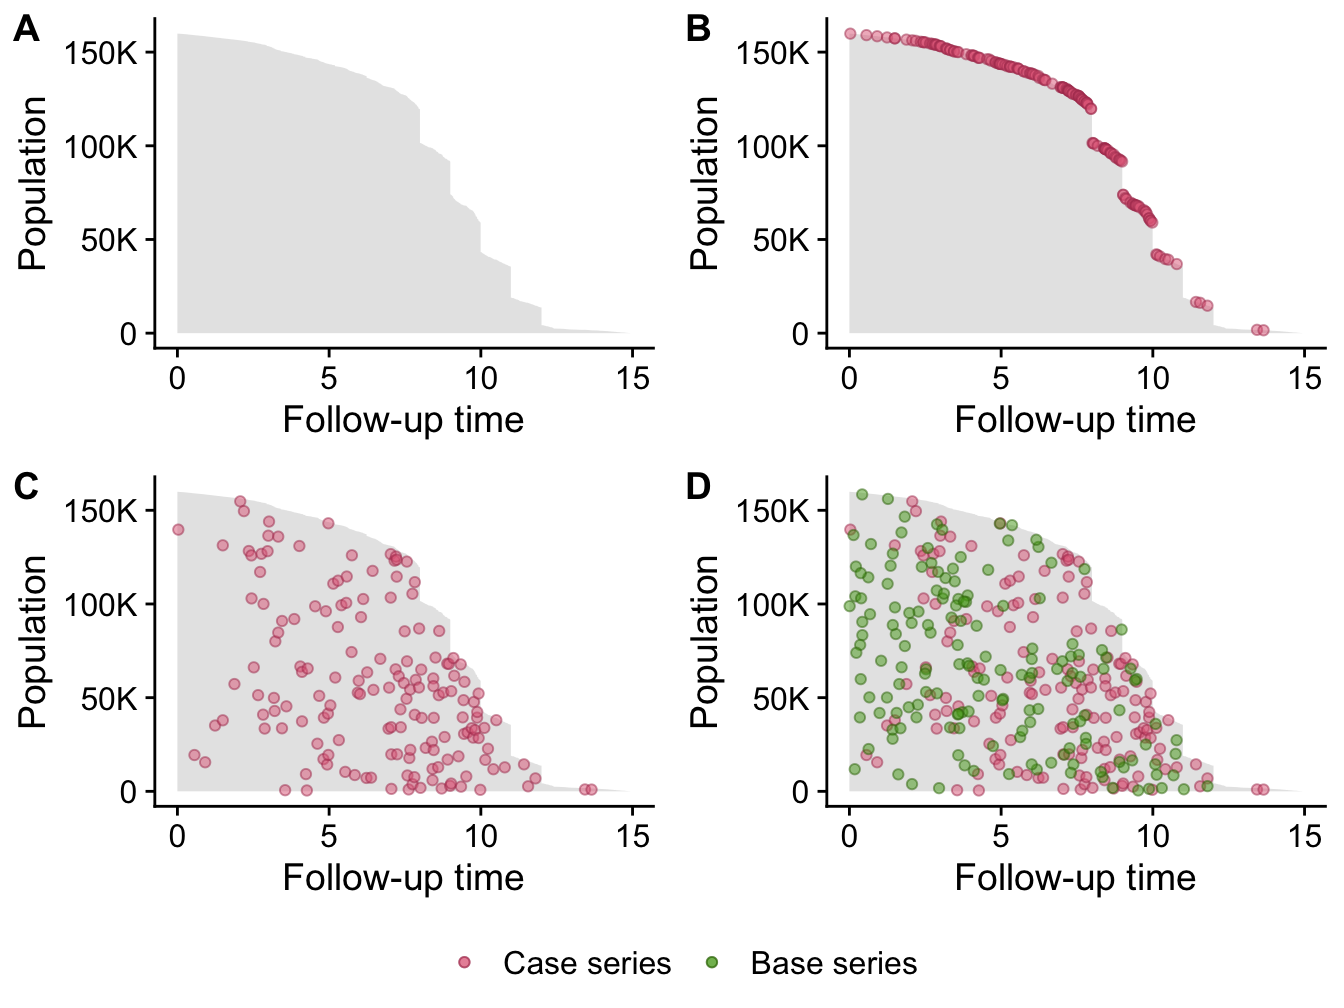
\includegraphics[width=\textwidth,keepaspectratio=true]{./plot-erspc-data-1} \caption{Population time plot for the ERSPC dataset. A: The gray area can be thought of as N=159,893 infinitely thin horizontal rectangles ordered by length of follow-up. B: The red points correspond to when death has occurred for any one of those infinitely thin rectangles. C: To improve visibility, these red points are randomly redistributed along their respective x-coordinates, providing a visualization of incidence density. More events are observed at later follow-up times, motivating the use of non-constant hazard models. D: The base series, a representative sample of the entire grey area, is represented by the green points.}\label{fig:plot-erspc-data}
\end{figure}

We then pass this object to the corresponding \texttt{plot} method:

\begin{verbatim}
plot(pt_object, add.base.series = TRUE)
\end{verbatim}

Figure \ref{fig:plot-erspc-data} depicts the process of creating a population-time plot. It is built sequentially by first adding a layer for the area representing the population time in gray (Figure \ref{fig:plot-erspc-data}A), with subjects having the least amount of observation time plotted at the top of the y-axis. We immediately notice a distinctive \emph{stepwise shape} in the population time area. This is due to the randomization of the Finnish cohorts which were carried out on January 1 of each of year from 1996 to 1999. Coupled with the uniform December 31 2006 censoring date, this led to large numbers of men with exactly 11, 10, 9 or 8 years of follow-up. Tracked backwards in time (i.e.~from right to left), the population-time plot shows the recruitment pattern from its beginning in 1991, and the January 1 entries in successive years. Tracked forwards in time (i.e.~from left to right), the plot for the first three years shows attrition due entirely to death (mainly from other causes). Since the Swedish and Belgian centres were the last to complete recruitment in December 2003, the minimum potential follow-up is three years. Tracked further forwards in time (i.e.~after year 3) the attrition is a combination of deaths and staggered entries. As we can see, population-time plots summarise a wealth of information about the study into a simple graph.

Next, layers for the case series and base series are added. The y-axis location of each case moment is sampled at random vertically on the plot to avoid having all points along the upper edge of the gray area (Figure \ref{fig:plot-erspc-data}B). By randomly distributing the cases, we can get a sense of the incidence density. In Figure \ref{fig:plot-erspc-data}C, we see that more events are observed at later follow-up times. Therefore, a constant hazard model would not be appropriate in this instance as it would overestimate the incidence earlier on in time, and underestimate it later on. Finally, the base series is sampled uniformly from the study base (Figure \ref{fig:plot-erspc-data}D). The reader should refer to the package vignettes for more examples and a detailed description of how to modify the aesthetics of a population-time plot.

\hypertarget{parametric-modeling}{%
\subsection{Parametric modeling}\label{parametric-modeling}}

The parametric modeling step was separated into three parts:

\begin{enumerate}
\def\labelenumi{\arabic{enumi}.}
\tightlist
\item
  case-base sampling;
\item
  estimation of the smooth hazard function;
\item
  estimation of the survival function.
\end{enumerate}

By separating the sampling and estimation functions, we allow the possibility of users implementing more complex sampling scheme (as described in Saarela (2016)), or more complex study designs (e.g.~time-varying exposure).

The sampling scheme selected for \texttt{sampleCaseBase} was described in Hanley \& Miettinen (2009): we first sample along the ``person'' axis, proportional to each individual's total follow-up time, and then we sample a moment uniformly over their follow-up time. This sampling scheme is equivalent to the following picture: imagine representing the total follow-up time of all individuals in the study along a single dimension, where the follow-up time of the next individual would start exactly when the follow-up time of the previous individual ends. Then the base series could be sampled uniformly from this one-dimensional representation of the overall follow-up time. In any case, the output is a dataset of the same class as the input, where each row corresponds to a person-moment. The covariate profile for each such person-moment is retained, and an offset term is added to the dataset. This output could then be used to fit a smooth hazard function, or for visualization of the base series.

Next, the fitting function \texttt{fitSmoothHazard} starts by looking at the class of the dataset: if it was generated from \texttt{sampleCaseBase}, it automatically inherited the class \texttt{cbData}. If the dataset supplied to \texttt{fitSmoothHazard} does not inherit from \texttt{cbData}, then the fitting function starts by calling \texttt{sampleCaseBase} to generate the base series. In other words, users can bypass \texttt{sampleCaseBase} altogether and only worry about the fitting function \texttt{fitSmoothHazard}.

The fitting function retains the familiar formula interface of \texttt{glm}. The left-hand side of the formula should be the name of the column corresponding to the event type. The right-hand side can be any combination of the covariates, along with an explicit functional form for the time variable. Note that non-proportional hazard models can be achieved at this stage by adding an interaction term involving time (cf.~Case Study 1 below). The offset term does not need to be specified by the user, as it is automatically added to the formula before calling \texttt{glm}.

To fit the hazard function, we provide several approaches that are available via the \texttt{family} parameter. These approaches are:

\begin{itemize}
\tightlist
\item
  \texttt{glm}: This is the familiar logistic regression.
\item
  \texttt{glmnet}: This option allows for variable selection using the elastic-net (Zou and Hastie 2005) penalty (cf.~Case Study 3). This functionality is provided through the \pkg{glmnet} package (Friedman, Hastie, and Tibshirani 2010).
\item
  \texttt{gam}: This option provides support for \emph{Generalized Additive Models} via the \CRANpkg{mgcv} package (Hastie and Tibshirani 1987).
\end{itemize}

In the case of multiple competing events, the hazard is fitted via multinomial regression as performed by the \CRANpkg{VGAM} package. We selected this package for its ability to fit multinomial regression models with an offset.

Once a model-fit object has been returned by \texttt{fitSmoothHazard}, all the familiar summary and diagnostic functions are available: \texttt{print}, \texttt{summary}, \texttt{predict}, \texttt{plot}, etc. Our package provides one more functionality: it computes risk functions from the model fit. For the case of a single event, it uses the familiar identity
\begin{equation}
S(t) = \exp\left(-\int_0^t \lambda(u;X) du\right). 
\label{eq:surv}
\end{equation}
The integral is computed using either the numerical or Monte-Carlo integration. The risk function (or cumulative distribution function) is then defined as
\begin{equation}
F(t) = 1 - S(t). \label{eq:CDF}
\end{equation}

For the case of a competing-event analysis, the event-specific risk is computed using the following procedure: first, we compute the overall survival function (i.e.~for all event types):

\[ S(t) = \exp\left(-\int_0^t \lambda(u;X) du\right),\qquad \lambda(t;X) = \sum_{j=1}^J \lambda_j(t;X).\]
From this, we can derive the cause-specific subdensities:

\[ f_j(t) = \lambda_j(t)S(t).\]

By integrating these subdensities, we obtain the cause-specific CI functions:

\[ CI_j(t) = \int_0^t f_j(u)du.\]
Again, the integrals are computed using either numerical integration (via the trapezoidal rule) or Monte Carlo integration. This option is controlled by the argument \texttt{method} of the \texttt{absoluteRisk} function.

Finally, the output from \texttt{absoluteRisk} can be passed to a method \texttt{confint} to compute confidence bands around the survival function, as described in the Theoretical Details section. These bands are only valid when \texttt{family\ =\ "glm"} as it relies on the asymptotic normality of the estimator. Currently, this is only available for the single-event setting.

\hypertarget{illustration-of-package}{%
\section{Illustration of package}\label{illustration-of-package}}

In this section, we illustrate the main functions of the \pkg{casebase} package through three case studies. Each one showcases a different type of analysis. First, we show how to model non-constant and non-proportional hazards through a flexible specification of time. Then we perform a competing risk analysis and compare our results with the Cox model and the Fine-Gray model. The third case study illustrates how to perform variable selection in high-dimensional datasets.

\hypertarget{case-study-1flexible-modeling-of-the-hazard-function}{%
\subsection{Case study 1---flexible modeling of the hazard function}\label{case-study-1flexible-modeling-of-the-hazard-function}}

For our first case study, we return to the ERSPC study and investigate the
differences in risk between the control and screening arms. Previous re-analyses
of these data suggest that the 20\% reduction in prostate cancer death due to
screening was an underestimate (Hanley 2010).
The estimated 20\% (from a proportional hazards model) did not account for
the delay between screening and the time the effect is expected to be observed.
As a result, the null effects in years 1--7 masked the substantial reductions
that began to appear from year 8 onward. This motivates the use of a
time-dependent hazard ratio which can easily be fit with the \pkg{casebase}
package by including an interaction term with time in the model. We fit a
flexible hazard by using a smooth function of time modeled with a penalized
cubic spline basis with 2 degrees of freedom (implemented in the
\texttt{survival::pspline} function). The model is fit using \texttt{fitSmoothHazard}
with the familiar formula interface:

\begin{verbatim}
fit <- fitSmoothHazard(DeadOfPrCa ~ pspline(Follow.Up.Time, df = 2) * ScrArm, 
                       data = ERSPC, ratio = 10)
\end{verbatim}

The output object from \texttt{fitSmoothHazard} inherits from the \texttt{singleEventCB}
and \texttt{glm} classes. For this reason, we can leverage the \texttt{summary}
method for \texttt{glm} objects to output a familiar summary of the results:

\begin{verbatim}
summary(fit) 
#> Fitting smooth hazards with case-base sampling
#> 
#> Sample size: 159893 
#> Number of events: 540 
#> Number of base moments: 5400 
#> ----
#> 
#> Call:
#> fitSmoothHazard(formula = DeadOfPrCa ~ pspline(Follow.Up.Time, 
#>     df = 2) * ScrArm, data = ERSPC, ratio = 10)
#> 
#> Deviance Residuals: 
#>    Min      1Q  Median      3Q     Max  
#> -1.168  -0.486  -0.414  -0.215   3.262  
#> 
#> Coefficients:
#>                                                        Estimate Std. Error
#> (Intercept)                                              -13.81       9.98
#> pspline(Follow.Up.Time, df = 2)1                           2.66      10.96
#> pspline(Follow.Up.Time, df = 2)2                           6.43       9.73
#> pspline(Follow.Up.Time, df = 2)3                           5.57      10.10
#> pspline(Follow.Up.Time, df = 2)4                           7.27       9.90
#> pspline(Follow.Up.Time, df = 2)5                           6.54      10.10
#> pspline(Follow.Up.Time, df = 2)6                          10.82      10.03
#> pspline(Follow.Up.Time, df = 2)7                         -11.74      30.13
#> ScrArmScreening group                                      9.22      13.35
#> pspline(Follow.Up.Time, df = 2)1:ScrArmScreening group    -9.25      14.85
#> pspline(Follow.Up.Time, df = 2)2:ScrArmScreening group    -9.80      12.97
#> pspline(Follow.Up.Time, df = 2)3:ScrArmScreening group    -9.04      13.54
#> pspline(Follow.Up.Time, df = 2)4:ScrArmScreening group    -9.39      13.23
#> pspline(Follow.Up.Time, df = 2)5:ScrArmScreening group   -10.65      13.55
#> pspline(Follow.Up.Time, df = 2)6:ScrArmScreening group    -8.86      13.46
#> pspline(Follow.Up.Time, df = 2)7:ScrArmScreening group   -11.58      36.92
#>                                                        z value Pr(>|z|)
#> (Intercept)                                              -1.38     0.17
#> pspline(Follow.Up.Time, df = 2)1                          0.24     0.81
#> pspline(Follow.Up.Time, df = 2)2                          0.66     0.51
#> pspline(Follow.Up.Time, df = 2)3                          0.55     0.58
#> pspline(Follow.Up.Time, df = 2)4                          0.73     0.46
#> pspline(Follow.Up.Time, df = 2)5                          0.65     0.52
#> pspline(Follow.Up.Time, df = 2)6                          1.08     0.28
#> pspline(Follow.Up.Time, df = 2)7                         -0.39     0.70
#> ScrArmScreening group                                     0.69     0.49
#> pspline(Follow.Up.Time, df = 2)1:ScrArmScreening group   -0.62     0.53
#> pspline(Follow.Up.Time, df = 2)2:ScrArmScreening group   -0.76     0.45
#> pspline(Follow.Up.Time, df = 2)3:ScrArmScreening group   -0.67     0.50
#> pspline(Follow.Up.Time, df = 2)4:ScrArmScreening group   -0.71     0.48
#> pspline(Follow.Up.Time, df = 2)5:ScrArmScreening group   -0.79     0.43
#> pspline(Follow.Up.Time, df = 2)6:ScrArmScreening group   -0.66     0.51
#> pspline(Follow.Up.Time, df = 2)7:ScrArmScreening group   -0.31     0.75
#> 
#> (Dispersion parameter for binomial family taken to be 1)
#> 
#>     Null deviance: 3619.1  on 5939  degrees of freedom
#> Residual deviance: 3359.1  on 5924  degrees of freedom
#> AIC: 3391
#> 
#> Number of Fisher Scoring iterations: 7
\end{verbatim}

As noted in the Theoretical Details section, the usual asymptotic results hold
for likelihood ratio tests built using case-base sampling models. Therefore, we
can easily test the significance of the spline term and its interaction with time:

\begin{verbatim}
anova(fit, test = "LRT")
#> Analysis of Deviance Table
#> 
#> Model: binomial, link: logit
#> 
#> Response: DeadOfPrCa
#> 
#> Terms added sequentially (first to last)
#> 
#> 
#>                                        Df Deviance Resid. Df Resid. Dev
#> NULL                                                    5939       3619
#> pspline(Follow.Up.Time, df = 2)         7    246.6      5932       3373
#> ScrArm                                  1      5.6      5931       3367
#> pspline(Follow.Up.Time, df = 2):ScrArm  7      7.9      5924       3359
#>                                        Pr(>Chi)    
#> NULL                                               
#> pspline(Follow.Up.Time, df = 2)          <2e-16 ***
#> ScrArm                                    0.018 *  
#> pspline(Follow.Up.Time, df = 2):ScrArm    0.343    
#> ---
#> Signif. codes:  0 '***' 0.001 '**' 0.01 '*' 0.05 '.' 0.1 ' ' 1
\end{verbatim}

Similarly, to compare different models (e.g.~time modeled linearly), we could
compute Akaike's Information Criterion (AIC) for each model.

\hypertarget{time-dependent-hazard-ratios}{%
\subsubsection{Time-dependent hazard ratios}\label{time-dependent-hazard-ratios}}

In what follows, the hazard ratio for a variable \(X\) is defined as

\[
\frac{\lambda\left(t | X=x_1, \mathbf{Z}=\mathbf{z} ; \widehat{\beta}\right)}{\lambda(t | X=x_0, \mathbf{Z}=\mathbf{z} ; \widehat{\beta})}
\]
where \(\lambda(t|\cdot;\widehat{\beta})\) is the hazard rate as a function of the
variable \(t\) (which is usually time, but can be any other continuous variable),
\(x_1\) is the value of \(X\) for the exposed group, \(x_0\) is the value of \(X\) for
the unexposed group, \(\mathbf{Z}\) are other covariates in the model which are
equal to \(\mathbf{z}\) in both the exposed and unexposed group,
and \(\widehat{\beta}\) are the estimated regression coefficients. As indicated by the
formula above, it is most instructive to plot the hazard ratio as a function of
a variable \(t\) only if there is an interaction between \(t\) and \(X\). Otherwise,
the resulting plot will simply be a horizontal line across time.

The \texttt{plot} method with \texttt{type="hr"} for objects of class
\texttt{singleEventCB} can be used to compute time-dependent hazard ratios and
confidence intervals. In Figure \ref{fig:interaction-ERSPC}, we show the
estimated hazard ratio and 95\% confidence interval for screening vs.~control
group as a function of time. Note that we must specify the covariate profile for
the reference group and times for the predicted hazards.

\begin{verbatim}
new_time <- seq(1, 12, by  = 0.1)
new_data <- data.frame(ScrArm = factor("Control group",
                                         levels = c("Control group","Screening group")),
                      Follow.Up.Time = new_time)
plot(fit, type = "hr", newdata = new_data,
     var = "ScrArm", xvar = "Follow.Up.Time", ci = TRUE)
\end{verbatim}

\begin{figure}[ht]
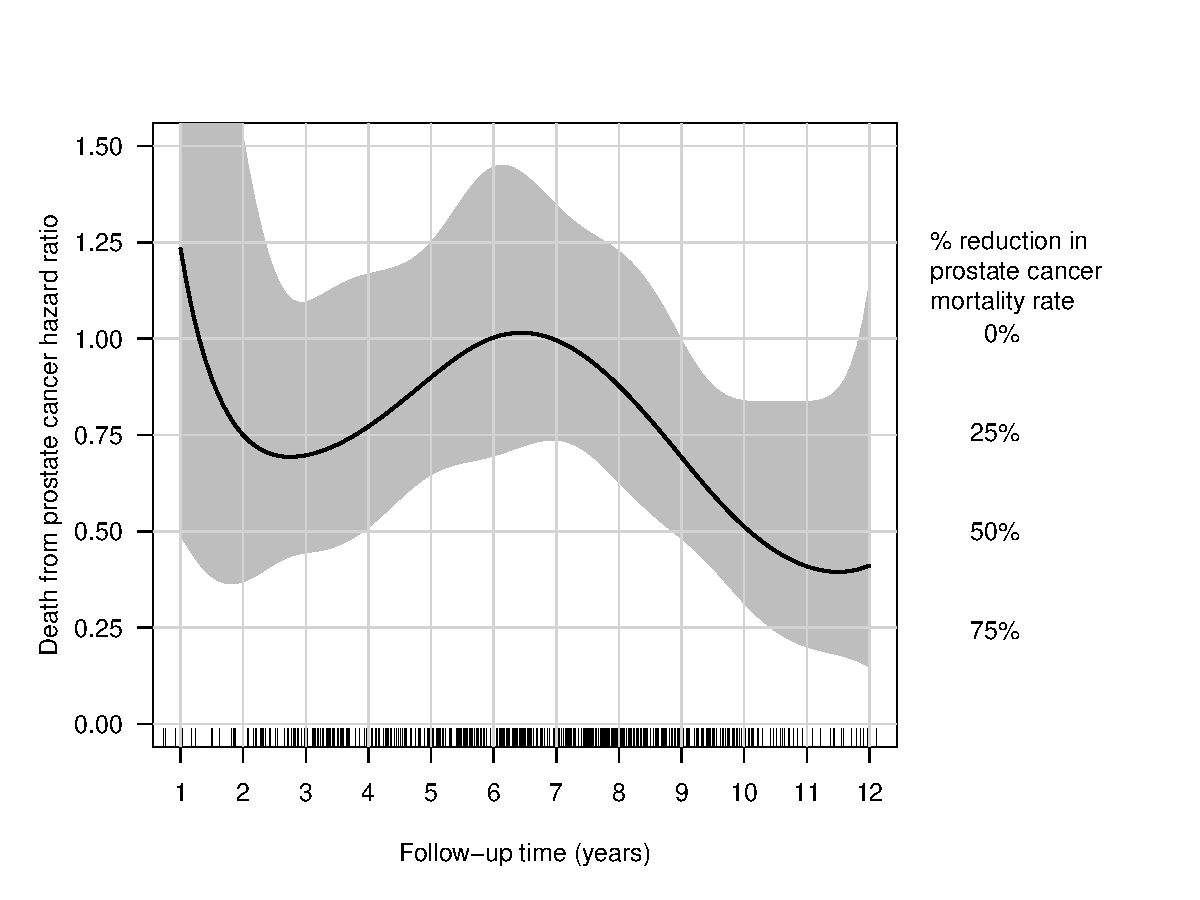
\includegraphics[width=\textwidth,keepaspectratio=true]{./interaction-ERSPC-1} \caption{Estimated hazard ratio and 95\% confidence interval for screening vs. control group as a function of time in the ERSPC dataset. Hazard ratios are estimated from fitting a parametric hazard model as a function of the interaction between a cubic pspline basis (df=2) of follow-up time and treatment arm. 95\% confidence intervals are calculated using the delta method. The plot shows that the effect of screening only begins to become statistically apparent by year 7. The 25-60\% reductions seen in years 8-12 of the study suggests a much higher reduction in prostate cancer due to screening than the single overall 20\% reported in the original article.}\label{fig:interaction-ERSPC}
\end{figure}

The plot shows that the effect of screening only becomes statistically apparent by year 7 and later. The 25-60\% reductions seen in years 8-12 of the study suggests a much higher reduction in prostate cancer due to screening than the single overall 20\% reported in the original article.

A more parsimonious model based on these results could be constructed as follows:

\[ \log \lambda\left(t \mid \mathbf{Z}\right) = \begin{cases} \alpha, &\quad t < t_0\\
\alpha + \beta Z(t - t_0), &\quad t \geq t_0\end{cases},\]
where \(t_0 \approx 7\) years. This model corresponds to a hazard ratio that is constant and equal to 1 until \(t = t_0\), after which it decreases exponentially. If we fix the value \(t_0\), we can easily implement this model using our package; for example:

\begin{verbatim}
fitSmoothHazard(DeadOfPrCa ~ as.integer(Follow.Up.Time >= t0) :
                    ScrArm : I(Follow.Up.Time - t0),
                data = ERSPC)
\end{verbatim}

Here, we use the binary variable \texttt{as.integer(Follow.Up.Time\ \textgreater{}=\ t0)} in order to write the two cases of our formula above in a more compact way. We also use the function \texttt{I()}, which allows us to specify new variables within the formula using normal \texttt{R} code. This is required, as otherwise the symbol \texttt{-} would be interpreted as a formula operator. Finally, the term \texttt{ScrArm\ :\ I(Follow.Up.Time\ -\ t0)} represents the product \(Z (t - t_0)\) in the equation above. We use the operator \texttt{:} instead of \texttt{*} in order to only include the interaction term, not the main effects.

Alternatively, the breakpoint \(t_0\) could also be estimated by combining case-base sampling with segmented regression. However, this extension is beyond the current scope of \texttt{casebase}.

\hypertarget{hazard-functions}{%
\subsubsection{Hazard functions}\label{hazard-functions}}

Modeling the hazard function directly allows us to easily visualize it with
the \texttt{plot} method and \texttt{type="hazard"} for objects of class \texttt{singleEventCB}.
We plot the hazard functions for both treatment arms in Figure \ref{fig:cs1hazard}.
The pattern we see is consistent with the population-time plot shown in Figure \ref{fig:plot-erspc-data}C, where more events are observed at later follow-up times.
The drop at the end can be explained by the fact that very few observations were followed for the entire 15 year period.

\begin{verbatim}
plot(fit, type = "hazard",
     hazard.params = list(xvar = "Follow.Up.Time",
                          by = "ScrArm"))
#> Conditions used in construction of plot
#> ScrArm: Control group / Screening group
#> offset: 0
\end{verbatim}

\begin{figure}[ht]
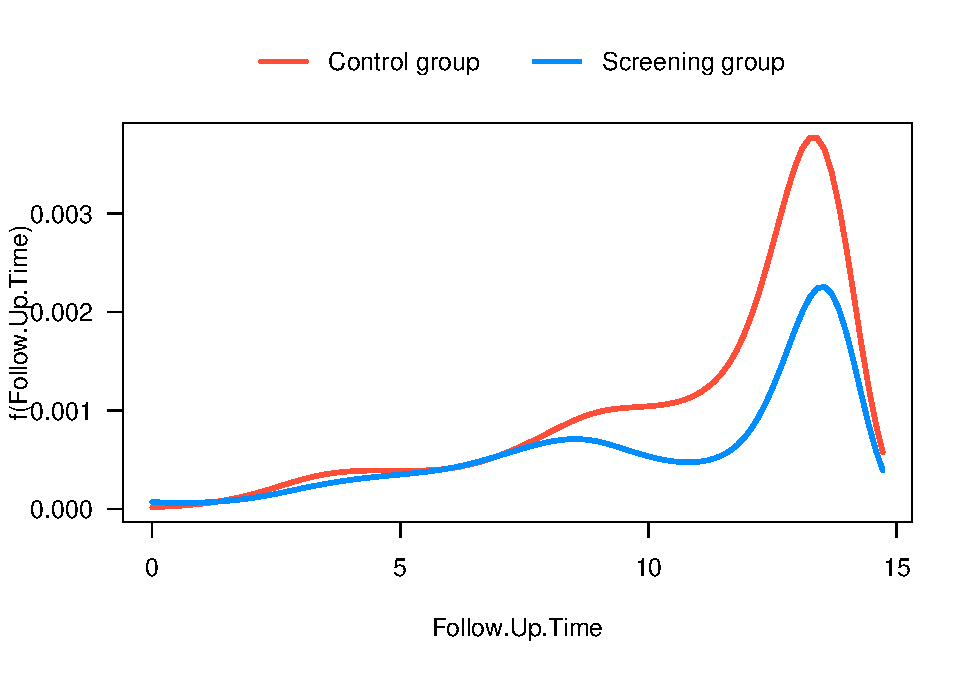
\includegraphics[width=\textwidth,keepaspectratio=true]{./cs1hazard-1} \caption{Estimated hazard functions for control and screening groups in the ERSPC dataset. Hazards are estimated from fitting a parametric model with casebase sampling as a function of the interaction between a cubic pspline basis (df=2) of follow-up time and treatment arm. The package vignettes provide a detailed description of how to plot hazard functions for any combination of covariates along with confidence bands.}\label{fig:cs1hazard}
\end{figure}

\hypertarget{absolute-risk}{%
\subsubsection{Absolute risk}\label{absolute-risk}}

Next, the \texttt{absoluteRisk} function takes as input the \texttt{singleEventCB} object and returns a matrix where each column corresponds to the covariate profiles specified in the \texttt{newdata} argument, and each row corresponds to time points specified by the \texttt{time} argument:

\begin{verbatim}
new_data <- data.frame(ScrArm = c("Control group", "Screening group"))
new_time <- seq(0,14,0.1)
risk <- absoluteRisk(fit, time = new_time, newdata = new_data)
\end{verbatim}

We can subsequently compute confidence intervals for the risk function using
the method \texttt{confint.absRiskCB}:

\begin{verbatim}
conf_ints <- confint(risk, fit)
head(conf_ints)
#>   time estimate conf.low conf.high      cov_prof
#> 1  0.0  0.0e+00  0.0e+00   0.0e+00 Control group
#> 2  0.1  1.8e-06  1.9e-07   1.2e-05 Control group
#> 3  0.2  3.9e-06  4.8e-07   2.2e-05 Control group
#> 4  0.3  6.1e-06  9.0e-07   3.2e-05 Control group
#> 5  0.4  8.7e-06  1.5e-06   4.1e-05 Control group
#> 6  0.5  1.2e-05  2.3e-06   5.0e-05 Control group
\end{verbatim}

In Figure \ref{fig:erspc-cif-conf}, we see the 95\% confidence bands around the estimates.
We also overlay the Kaplan-Meier curves as a reference.

\begin{figure}[ht]
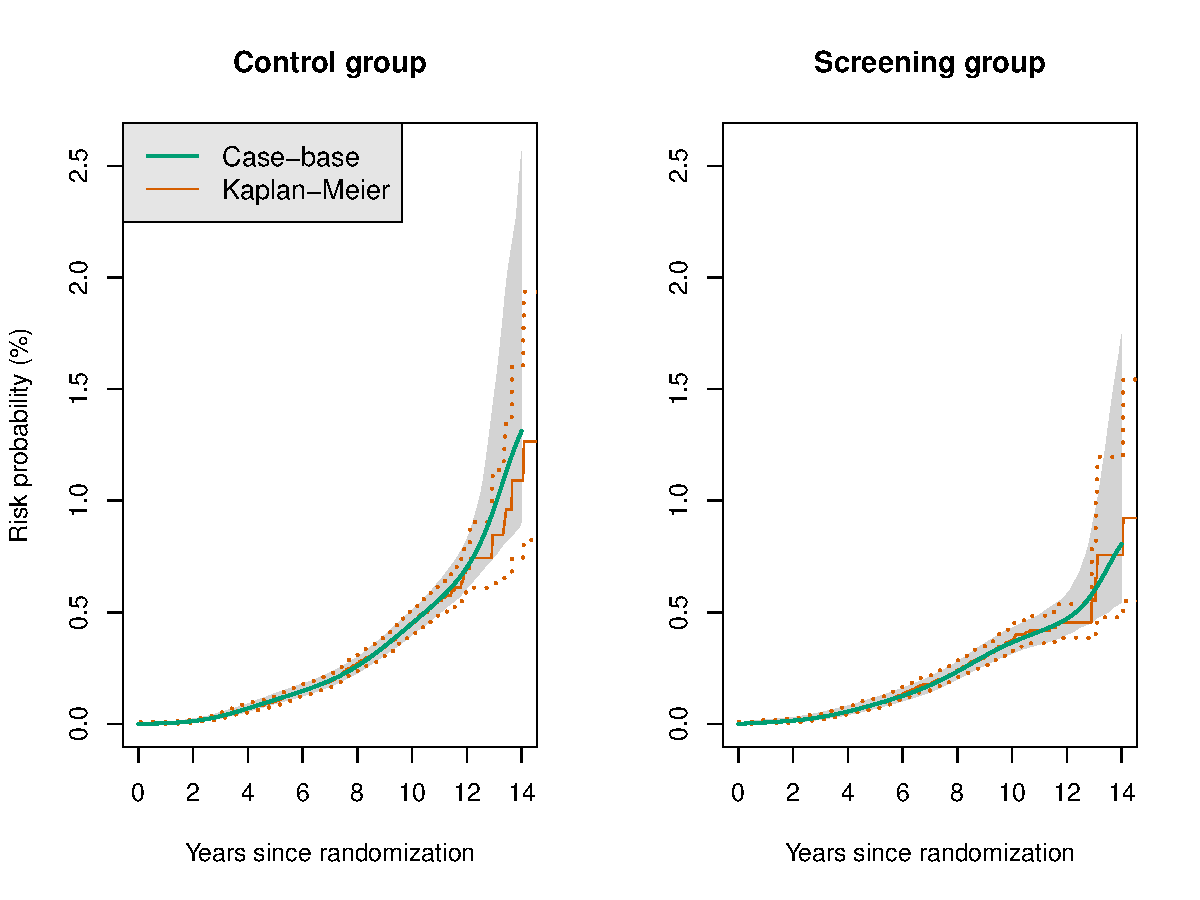
\includegraphics[width=\textwidth,keepaspectratio=true]{./erspc-cif-conf-1} \caption{Risk function estimates for control and screening groups in the ERSPC data using case-base sampling and Kaplan-Meier, along with 95\% confidence bands. The smooth curve (case-base sampling) vs. step function (Cox model) highlight one of the main differences between the two approaches. The larger confidence bands in the later years is due to the relatively few number of individuals who were followed for more than 12 years.}\label{fig:erspc-cif-conf}
\end{figure}

\hypertarget{case-study-2competing-risk-analysis}{%
\subsection{Case study 2---competing risk analysis}\label{case-study-2competing-risk-analysis}}

In this case study, we show how case-base sampling can be used in the context of a competing risk analysis. For illustrative purposes, we use the same data that was used in Scrucca \emph{et al} (2010). The data was downloaded from the first author's website, and it is now available as part of the \pkg{casebase} package.

The data contains information on 177 patients who received a stem-cell transplant for acute leukemia. The event of interest is relapse, but other competing causes (e.g.~death, progression, graft failure, graft-versus-host disease) were also recorded. Several covariates were captured at baseline: sex, disease type (acute lymphoblastic or myeloblastic leukemia, abbreviated as ALL and AML, respectively), disease phase at transplant (Relapse, CR1, CR2, CR3), source of stem cells (bone marrow and peripheral blood, coded as BM+PB, or only peripheral blood, coded as PB), and age.

First, we look at a population-time plot to visualize the incidence density of both relapse and the competing events. In Figure \ref{fig:compPop}, failure times are highlighted on the plot using red dots for the event of interest and blue dots for competing events. In this plot, we see evidence of a non-constant hazard function: the density of points is larger at the beginning of follow-up than at the end.

\begin{figure}[ht]
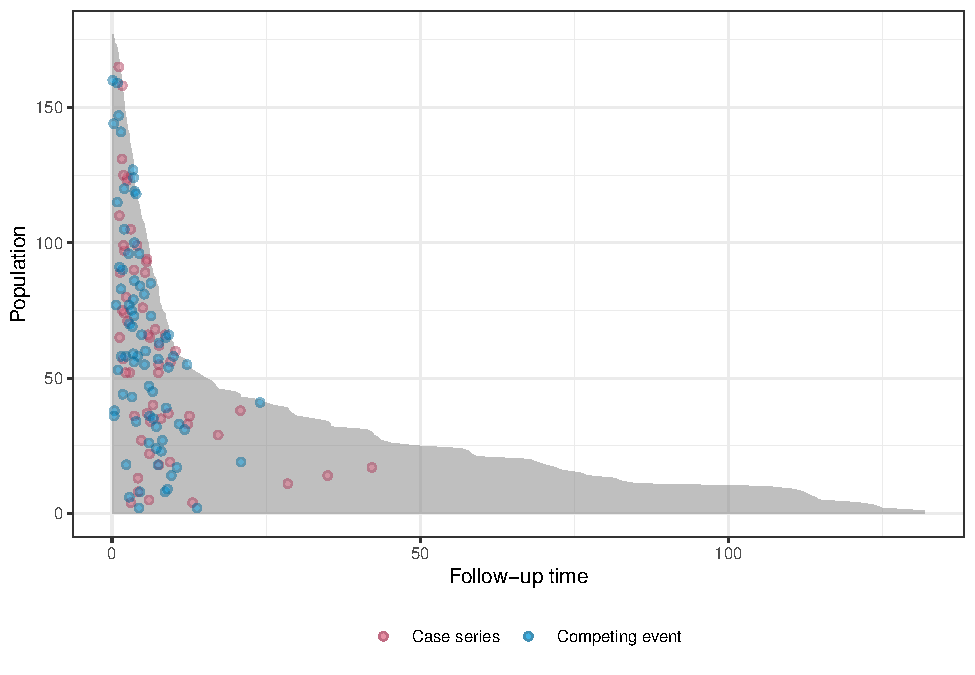
\includegraphics[width=\textwidth,keepaspectratio=true]{./compPop-1} \caption{Population-time plot for the stem-cell transplant study with both relapse and competing events. The area representing the population time is shown in gray, with subjects having the least amount of observation time plotted at the top of the y-axis. The y-axis location of each case series and competing event moment is sampled at random vertically on the plot to avoid having all points along the upper edge of the gray area. The density of points at the beginning of follow-up relative to the end indicates a non-constant hazard function.}\label{fig:compPop}
\end{figure}

Our main objective is to compute the cumulative incidence of relapse for a given set of covariates. We start by fitting a smooth hazard to the data using a linear term for time:

\begin{verbatim}
model_cb <- fitSmoothHazard(
  Status ~ ftime + Sex + D + Phase + Source + Age,
  data = bmtcrr,
  ratio = 100,
  time = "ftime"
)
\end{verbatim}

We want to compare our hazard ratio estimates to that obtained from a Cox regression (using the \pkg{survival} package version 3.2-13).

\begin{verbatim}
library(survival)
# Prepare data for coxph
bmtcrr_cox <- transform(bmtcrr, 
                        id = seq_len(nrow(bmtcrr)),
                        Status = factor(Status))

model_cox <- coxph(Surv(ftime, Status) ~ Sex + D + Phase + Source + Age,
                   data = bmtcrr_cox, id = id)
\end{verbatim}

\begin{table}

\caption{\label{tab:bmtcrr-cis}Estimates and confidence intervals for the hazard ratios for each coefficient. Both estimates from case-base sampling and Cox regression are presented.}
\centering
\begin{tabular}[t]{lrlrl}
\toprule
\multicolumn{1}{c}{ } & \multicolumn{2}{c}{Case-Base} & \multicolumn{2}{c}{Cox} \\
\cmidrule(l{3pt}r{3pt}){2-3} \cmidrule(l{3pt}r{3pt}){4-5}
Covariates & HR & 95\% Conf. & HR & 95\% Conf.\\
\midrule
Sex & 0.73 & (0.42, 1.27) & 0.68 & (0.39, 1.21)\\
Disease & 0.54 & (0.3, 0.98) & 0.52 & (0.28, 0.94)\\
Phase (CR2 vs. CR1) & 1.19 & (0.48, 2.97) & 1.21 & (0.47, 3.09)\\
Phase (CR3 vs. CR1) & 1.44 & (0.37, 5.64) & 1.67 & (0.46, 6.08)\\
Phase (Relapse vs. CR1) & 4.22 & (1.95, 9.12) & 4.55 & (1.98, 10.46)\\
\addlinespace
Source & 1.46 & (0.48, 4.46) & 1.46 & (0.47, 4.53)\\
Age & 0.99 & (0.97, 1.02) & 0.99 & (0.97, 1.02)\\
\bottomrule
\end{tabular}
\end{table}

From the fit object, we can extract both the hazard ratios and their corresponding confidence intervals. These quantities appear in Table \ref{tab:bmtcrr-cis}. As we can see, the type of disease corresponds to a significant hazard ratio: the hazard for AML is about half that for ALL. Moreover, being in relapse at transplant is associated with a hazard ratio of 4.22 when compared to CR1.

Given the estimate of the hazard functions obtained using case-base sampling, we can compute the cumulative incidence curve for a fixed covariate profile. We perform this computation for a 35 year old woman who received a stem-cell transplant from peripheral blood at relapse. We compare the absolute risk curve for such a woman with ALL with that for a similar woman with AML.

Next, we compare our estimates to that obtained from a corresponding Fine-Gray model (1999). The Fine-Gray model is a semiparametric model for the cause-specific \emph{subdistribution hazard}, i.e.~the function \(d_j(t)\) such that
\[CI_j(t) = 1 - \exp\left( - \int_0^t d_j(u) \textrm{d}u \right),\]
where \(CI_j(t)\) is the cause-specific CI. The Fine-Gray model allows to directly assess the effect of a covariate on the subdistribution hazard, as opposed to the cause-specific hazard. For the computation, we use the \CRANpkg{timereg} package (Thomas H. Scheike and Zhang 2011):

\begin{verbatim}
library(timereg)
model_fg <- comp.risk(Event(ftime, Status) ~ const(Sex) + const(D) +
                        const(Phase) + const(Source) + const(Age),
                      data = bmtcrr, cause = 1, model = "fg")

# Estimate CI curve
risk_fg <- predict(model_fg, newdata, times = time_points)
\end{verbatim}

We can also estimate the CI for relapse using the Cox model and the Aalen-Johansen estimator:

\begin{verbatim}
# Estimate absolute risk curve
risk_cox <- survfit(model_cox, newdata = newdata)
\end{verbatim}

\begin{figure}[ht]
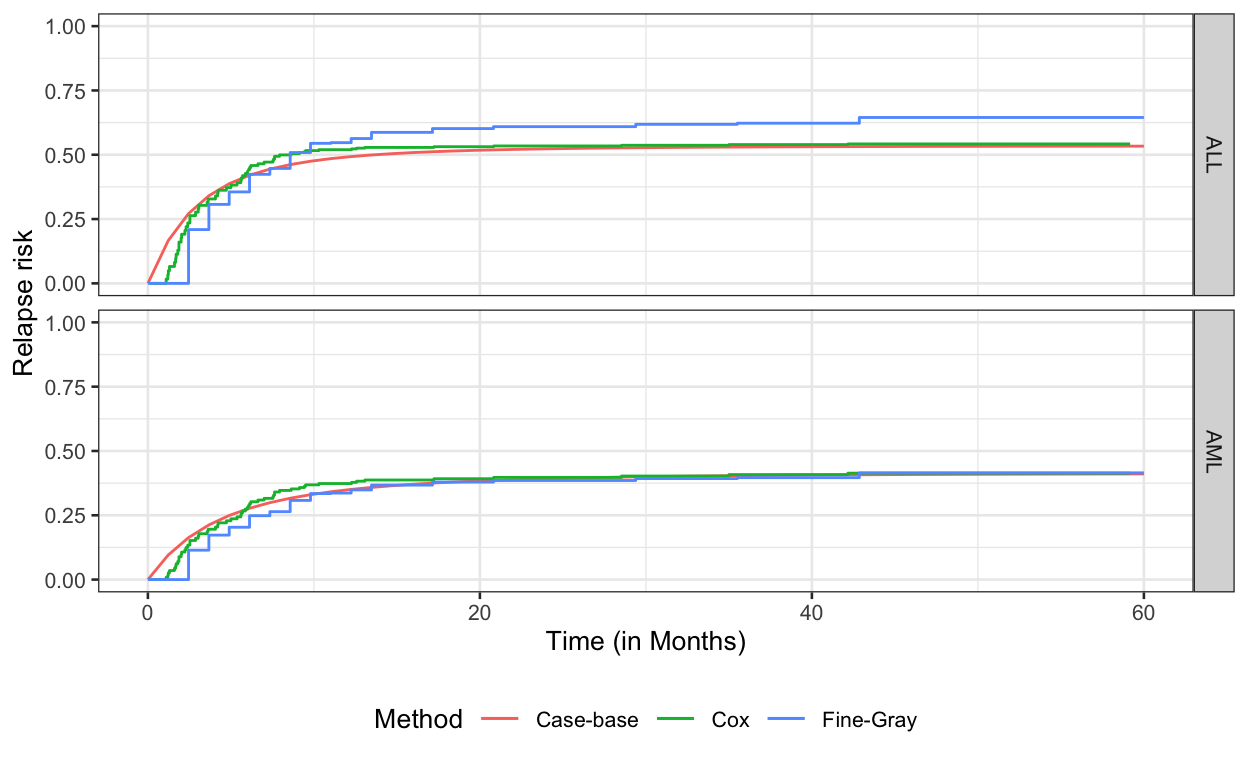
\includegraphics[width=\textwidth,keepaspectratio=true]{./compAbsrisk-1} \caption{Cumulative Incidence curve for a fixed covariate profile and the two disease groups. The estimate obtained from case-base sampling is compared to the Fine-Gray and Aalen-Johansen estimates. In general, the three approaches agree quite well for AML, while there seems to be a difference of about 5\% between the Fine-Gray curve and the curves estimated using case-base sampling and Cox regression for ALL. However, this difference does not appear to be significant as the curve from case-base sampling is contained within a 95\% confidence band around the Fine-Gray absolute risk curve (figure not shown).}\label{fig:compAbsrisk}
\end{figure}

Figure \ref{fig:compAbsrisk} shows the CI curves for all three models. As we can see, all three approaches agree quite well for AML; however, for ALL, there seems to be a difference of about 5\% between the Fine-Gray curve and the curves estimated using case-base sampling and Cox regression. This difference does not appear to be significant: the curve from case-base sampling is contained within a 95\% confidence band around the Fine-Gray absolute risk curve (figure not shown).

\hypertarget{case-study-3variable-selection}{%
\subsection{Case study 3---variable selection}\label{case-study-3variable-selection}}

For the third case study, we show how \pkg{casebase} can also be used for variable selection through regularized estimation of the hazard function as given by Equation \eqref{eq:penest}. We note that this is different than the semiparametric model Coxnet, which regularizes the Cox partial likelihood. To illustrate this functionality, we use the dataset from the Study to Understand Prognoses Preferences Outcomes and Risks of Treatment (SUPPORT) (Knaus et al. 1995).\footnote{The original data is available online from the Department of Biostatistics at Vanderbilt University: \url{https://biostat.app.vumc.org/wiki/Main/SupportDesc}} The SUPPORT dataset tracks death in five American hospitals within individuals who are considered seriously ill.~The cleaned and imputed data consists of 9104 observations and 30 variables, and it is available as part of the \pkg{casebase} package. In the comparisons below, all covariates except \texttt{sps} and \texttt{aps} were used. These two variables correspond to scores for predicting the outcome that were developed as part of the original study. For more information about this dataset, the reader is encouraged to look at the documentation in our package.

For our penalized case-base model, we opt for the natural log of time which corresponds to a Weibull distribution. For fitting the penalized hazard, we use \texttt{fitSmoothHazard.fit}, which is a matrix interface to the \texttt{fitSmoothHazard} function. The \texttt{fitSmoothHazard} and \texttt{fitSmoothHazard.fit} functions sample the case and base series, calculate the required offset, and transform the data to match the expected input of the \pkg{glmnet} package. The penalized logistic regression is then fit for multiple values of the tuning parameter using the function \texttt{glmnet::cv.glmnet} and the binomial family. To \texttt{fitSmoothHazard.fit}, we supply both a matrix \texttt{y} containing the time and event variables, and a matrix \texttt{x} containing all other covariates. We apply the lasso penalty by setting \texttt{alpha\ =\ 1} and assign a \texttt{penalty.factor} (\(w_j\); cf.~Equation \eqref{eq:penest}) of 0 to the time variable to ensure it is in the selected model. We compare our approach to both Cox regression, and lasso penalized Cox regression (fitted via the \pkg{glmnet} package and using the Cox family).

To compare the performance of our models, we split the data into 95\% training and 5\% test sets. To assess both discrimination and calibration, we use a time-dependent version of the classical Brier score that is adjusted for censoring (Graf et al. 1999). The Brier score can be used with both parametric and semi-parametric models. We use the \pkg{riskRegression} package to compute these scores for all models.

\begin{verbatim}
# Create matrices for inputs
x <- model.matrix(death ~ . - d.time - aps - sps, 
                  data = train)[, -c(1)] # Remove intercept
y <- data.matrix(subset(train, select = c(d.time, death)))

# Regularized logistic regression to estimate hazard
pen_cb <- casebase::fitSmoothHazard.fit(x, y,
  family = "glmnet",
  time = "d.time", event = "death",
  formula_time = ~ log(d.time), alpha = 1,
  ratio = 10, standardize = TRUE,
  penalty.factor = c(0, rep(1, ncol(x)))
)
\end{verbatim}

In Figure \ref{fig:cs3lolliPlot}, we show the coefficient estimates for covariates that we selected by both penalized Cox and penalized case-base. We note that both penalized approaches produce similar results. We can also clearly see the shrinkage effect owing to the \(\ell_1\) penalty.

\begin{figure}[ht]
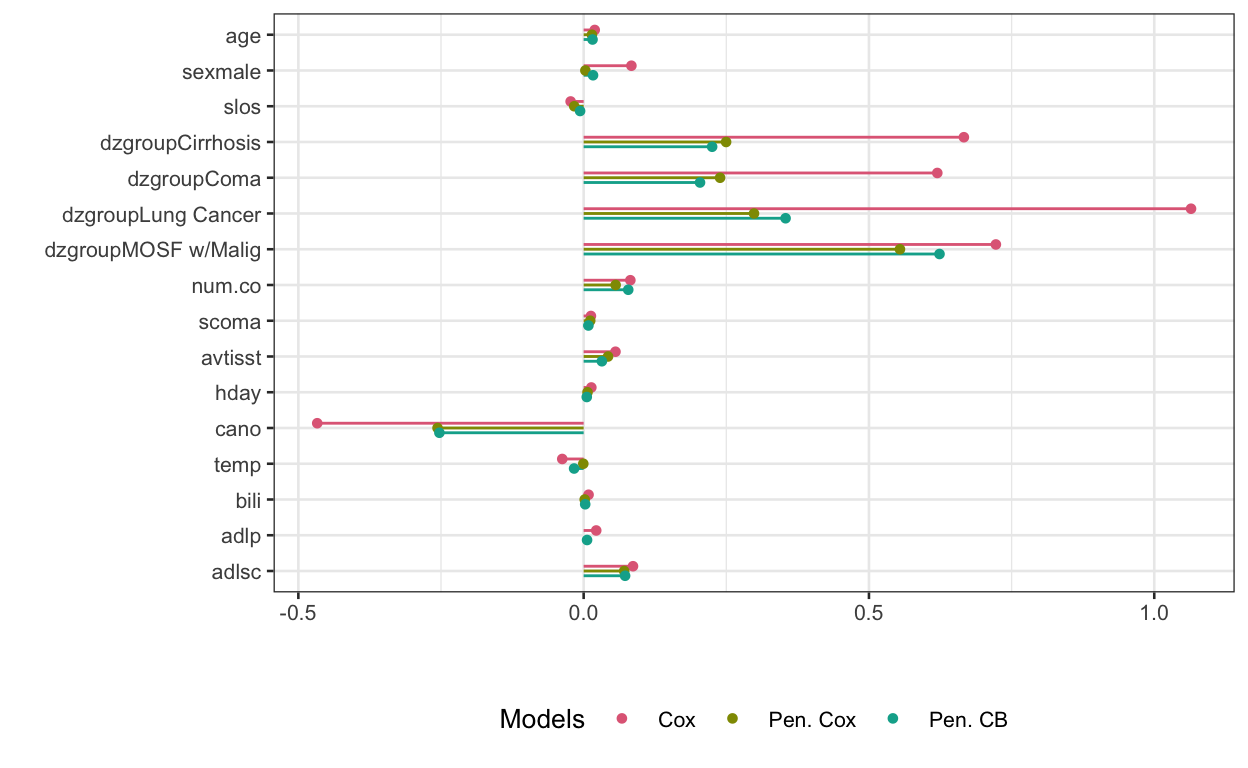
\includegraphics[width=\textwidth,keepaspectratio=true]{./cs3lolliPlot-1} \caption{Coefficient estimates from the Cox model (Cox), penalized Cox model using the glmnet package (Pen. Cox), and our approach using penalized case-base sampling (Pen. CB). Only the covariates that were selected by both penalized approaches are shown. The shrinkage of the coefficient estimates for Pen. Cox and Pen. CB occurs due to the $\ell_1$ penalty.}\label{fig:cs3lolliPlot}
\end{figure}

We then compare the risk estimation over the test set. The predicted probabilities for each test set observation are averaged, resulting in the absolute risk curves shown in Figure \ref{fig:cs3FinalBrier}A. The Kaplan-Meier curve is calculated on the test set only. We see minimal differences between the four approaches across follow-up-time. Note that the apparent smoothness of the Cox and penalized Cox curves is due to the large number of observations in the training set, which is used to derive the Breslow estimate of the baseline hazard. As described above, we compare the performance between the models by computing the Brier scores over time. In Figure \ref{fig:cs3FinalBrier}B, we see that the adjusted models all perform similarly, outperforming the Kaplan-Meier estimate.

\begin{figure}[ht]
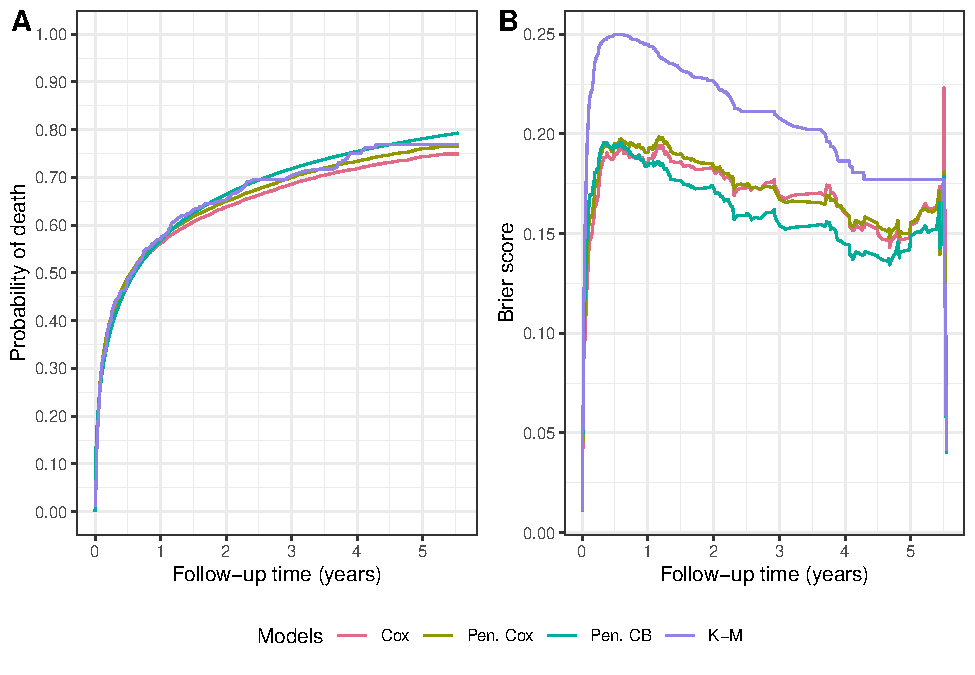
\includegraphics[width=\textwidth,keepaspectratio=true]{./cs3FinalBrier-1} \caption{Comparison of Cox regression (Cox), penalized Cox regression (Pen. Cox), penalized case-base sampling estimation (Pen. CB), and Kaplan-Meier (K-M). (A) Probability of death as a function of follow-up time which is the average of the predicted probabilities for each test set observation. The Kaplan-Meier curve is calculated on the test set only. We see minimal differences between the four approaches across follow-up-time for the absolute risk curves. Note that the apparent smoothness of the Cox and penalized Cox curves is due to the large number of observations in the training set, which is used to derive the Breslow estimate of the baseline hazard. (B) Brier score as a function of follow-up time, where a lower score corresponds to better performance. We see that the adjusted models all perform similarly, outperforming the Kaplan-Meier estimate.}\label{fig:cs3FinalBrier}
\end{figure}

\hypertarget{discussion}{%
\section{Discussion}\label{discussion}}

In this article, we presented the R package \pkg{casebase}, which provides functions for fitting smooth parametric hazards and estimating risk functions using case-base sampling. Our package also provides several functions to produce graphical summaries of the data and the results. We outlined the theoretical underpinnings of the approach, we provided details about our implementation, and we illustrated the merits of the case-base framework and the package through three case studies.

As a methodological framework, case-base sampling is very flexible. Some of this flexibility has been explored before in the literature: for example, Saarela and Hanley (2015) used case-base sampling to model a time-dependent exposure variable in a vaccine safety study. As another example, Saarela and Arjas (2015) combined case-base sampling and a Bayesian non-parametric framework to compute individualized risk assessments for chronic diseases. In the case studies above, we further explored this flexibility along two fronts. On the one hand, we showed how splines could be used as part of the linear predictor to model the effect of time on the hazard. This strategy yielded estimates of the survival function that were qualitatively similar to semiparametric estimates derived from Cox regression; however, case-base sampling led to estimates of the survival function that \emph{vary smoothly in time} and are thus easier to interpret. On the other hand, we also displayed the flexibility of case-base sampling by showing how it could be combined with penalized logistic regression to perform variable selection. Furthermore, the second case study showed how case-base sampling can be applied to competing risks settings. It should be noted that the three case studies presented above only considered covariates that were fixed at baseline. In one of the package vignettes, we use the Stanford Heart Transplant data Crowley and Hu (1977) to show how case-base sampling can also be used in the context of time-dependent exposure. In this study, the exposure period was defined as the week following vaccination. Hence, the main covariate of interest, i.e.~exposure to the vaccine, was changing over time. In this context, case-base sampling offers an efficient alternative to nested case-control designs or self-matching.

Even though we did not illustrate it in this article, case-base sampling can also be combined with the framework of \emph{generalized additive models}. This functionality has already been implemented in the package. Similarly, case-base sampling can be combined with quasi-likelihood estimation to fit survival models that can account for the presence of over-dispersion. All of these examples illustrate how the case-base sampling framework in general, and the package \pkg{casebase} in particular, allows the user to fit a broad and flexible family of survival functions.

Poisson regression can also be used to estimate the full hazard by discretizing time. However, this method requires user input on the number of intervals, or equivalently, on the cut points. This choice made by the user can have a significant impact on the model. Small intervals may result in many empty, non-informative bins. This may cause convergence issues for the Newton-Raphson procedure (Kalbfleisch and Prentice 2011). If the intervals are too wide, the nonlinear trends that are present in the hazard may be masked. Rather than discretizing time like in Poisson regression, case-base sampling provides a continuous-time approach to using GLMs for estimating hazard functions.

As presented in Hanley \& Miettinen (2009), case-base sampling is comprised of three steps: 1) sampling a case series and a base series from the study; 2) fit the log-hazard as a linear function of predictors (including time); and 3) use the fitted hazard to estimate the risk function. Accordingly, our package provides functions for each step. Moreover, the simple interface of the \texttt{fitSmoothHazard} function resembles the \texttt{glm} interface. This interface should look familiar to new users. Our modular approach also provides a convenient way to extend our package for new sampling or fitting strategies.

In the case studies above, we compared the performance of case-base sampling with that of Cox regression and Fine-Gray models. In terms of function interface, \pkg{casebase} uses a formula interface that is closer to that of \texttt{glm}, in that the event variable is the only variable appearing on the left-hand side of the formula. By contrast, both \texttt{survival::coxph} and \texttt{timereg::comp.risk} use arrays that capture both the event type and time. Both approaches to modeling yield user-friendly code. However, in terms of output, both approaches differ significantly. Case-base sampling produces smooth hazards and smooth survival curves, whereas Cox regression and Fine-Gray models produce stepwise CIs and never explicitly model the hazard function. Qualitatively, we showed that by using splines in the linear predictor, all three models yielded similar curves.

Our choice of modeling the log-hazard as a linear function of covariates allows us to develop a simple computational scheme for estimation. However, as a downside, it does not allow us to model location and scale parameters separately like the package \pkg{flexsurv}. For example, if we look at the Weibull distribution as parametrised in \texttt{stats::pweibull}, the log-hazard function is given by
\[ \log \lambda(t; \alpha, \beta) = \left[\log(\alpha/\beta) - (\alpha - 1)\log(\beta)\right] + (\alpha - 1)\log t,\]
where \(\alpha,\beta\) are shape and scale parameters, respectively. Unlike \pkg{casebase}, the approach taken by \pkg{flexsurv} also allows the user to model the scale parameter as a function of covariates. Of course, this added flexibility comes at the cost of interpretability: by modeling the log-hazard directly, the parameter estimates from \pkg{casebase} can be interpreted as estimates of log-hazard ratios. To improve the flexibility of \pkg{casebase} at capturing the scale of a parametric family, we could replace the logistic regression with its quasi-likelihood counterpart and therefore model over- and under-dispersion with respect to the logistic likelihood. We defer the study of the properties and performance of such a model to a future article.

Future work will look at some of the methodological extensions of case-base sampling. First, to assess the quality of the model fit, we would like to study the properties of the residuals (e.g.~Cox-Snell, martingale). More work needs to be done to understand these residuals in the context of the partial likelihood underlying case-base sampling. The resulting diagnostic tools could then be integrated in this package. Also, we are interested in extending case-base sampling to account for interval censoring. This type of censoring is very common in longitudinal studies, and many packages (e.g.~\pkg{SmoothHazard}, \pkg{survival} and \pkg{rstpm2}) provide functions to account for it. Again, we hope to include any resulting methodology as part of this package.

In future versions of the package, we also want to increase the complement of diagnostic and inferential tools that are currently available. For example, we would like to include more functions to compute calibration and discrimination statistics (e.g.~AUC) for our models. Saarela and Arjas (2015) also describe how to obtain a posterior distribution for the AUC from their model. Their approach could potentially be included in \pkg{casebase}. Finally, we want to provide more flexibility in how the case-base sampling is performed. This could be achieved by adding a \texttt{hazard} argument to the function \texttt{sampleCaseBase}. In this way, users could specify their own sampling mechanism. For example, they could provide a hazard that gives sampling probabilities that are proportional to the cardiovascular disease event rate given by the Framingham score (Saarela and Arjas 2015).

In conclusion, we presented the R package \pkg{casebase} which implements case-base sampling for fitting parametric survival models and for estimating smooth survival functions using the framework of generalized linear models. We strongly believe that its flexibility and its foundation on the familiar logistic regression model will make it appealing to new and established practitioners. The \pkg{casebase} package is freely available from the Comprehensive R Archive Network at \url{https://cran.r-project.org/package=casebase}. Interested users can visit \url{http://sahirbhatnagar.com/casebase/} for detailed package documentation and vignettes.

\hypertarget{acknowledgments}{%
\section{Acknowledgments}\label{acknowledgments}}

We would like to thank the anonymous reviewers for their insightful comments and criticisms. We would also like to thank Yi Yang for helpful discussions on penalized regression models. Bhatnagar (RGPIN-2020-05133) and Turgeon (RGPIN-2021-04073) both gratefully acknowledge funding via a Discovery Grant from the Natural Sciences and Engineering Research Council of Canada (NSERC), RGPIN.

\hypertarget{references}{%
\section*{References}\label{references}}
\addcontentsline{toc}{section}{References}

\hypertarget{refs}{}
\begin{CSLReferences}{1}{0}
\leavevmode\vadjust pre{\hypertarget{ref-aalen2008survival}{}}%
Aalen, Odd, Ornulf Borgan, and Hakon Gjessing. 2008. \emph{Survival and Event History Analysis: A Process Point of View}. Springer Science \& Business Media.

\leavevmode\vadjust pre{\hypertarget{ref-survTaskView}{}}%
Allignol, Arthur, and Aurelien Latouche. 2019. {``CRAN Task View: Survival Analysis.''} \emph{CRAN Task View: Survival Analysis}. \url{https://cran.r-project.org/web/views/Survival.html}.

\leavevmode\vadjust pre{\hypertarget{ref-arjas1987logistic}{}}%
Arjas, Elja, and Pentti Haara. 1987. {``A Logistic Regression Model for Hazard: Asymptotic Results.''} \emph{Scandinavian Journal of Statistics}, 1--18.

\leavevmode\vadjust pre{\hypertarget{ref-casebase-package}{}}%
Bhatnagar, Sahir, Maxime Turgeon, Jesse Islam, Olli Saarela, and James Hanley. 2021. \emph{Casebase: Fitting Flexible Smooth-in-Time Hazards and Risk Functions via Logistic and Multinomial Regression}. \url{https://CRAN.R-project.org/package=casebase}.

\leavevmode\vadjust pre{\hypertarget{ref-breslow1972discussion}{}}%
Breslow, NE. 1972. {``Discussion of the Paper by {Dr Cox} Cited Below.''} \emph{Journal of the Royal Statistical Society: Series B (Methodological)} 34: 187--220.

\leavevmode\vadjust pre{\hypertarget{ref-copenhagen2012needs}{}}%
Carstensen, Bendix. 2019. {``Who Needs the Cox Model Anyway.''} \url{http://bendixcarstensen.com/WntCma.pdf}.

\leavevmode\vadjust pre{\hypertarget{ref-clark1971cardiac}{}}%
Clark, David A, Edward B Stinson, Randall B Griepp, John S Schroeder, Norman E Shumway, and Donald Harrison. 1971. {``Cardiac Transplantation in Man.''} \emph{Annals of Internal Medicine} 75 (1): 15--21.

\leavevmode\vadjust pre{\hypertarget{ref-clements_liu}{}}%
Clements, Mark, and Xing-Rong Liu. 2019. \emph{Rstpm2: Smooth Survival Models, Including Generalized Survival Models}. \url{https://CRAN.R-project.org/package=rstpm2}.

\leavevmode\vadjust pre{\hypertarget{ref-crowley1977covariance}{}}%
Crowley, John, and Marie Hu. 1977. {``Covariance Analysis of Heart Transplant Survival Data.''} \emph{Journal of the American Statistical Association} 72 (357): 27--36.

\leavevmode\vadjust pre{\hypertarget{ref-efron1988logistic}{}}%
Efron, Bradley. 1988. {``Logistic Regression, Survival Analysis, and the Kaplan-Meier Curve.''} \emph{Journal of the American Statistical Association} 83 (402): 414--25.

\leavevmode\vadjust pre{\hypertarget{ref-efron1994introduction}{}}%
Efron, Bradley, and Robert J Tibshirani. 1994. \emph{An Introduction to the Bootstrap}. CRC press.

\leavevmode\vadjust pre{\hypertarget{ref-fine1999proportional}{}}%
Fine, Jason P, and Robert J Gray. 1999. {``A Proportional Hazards Model for the Subdistribution of a Competing Risk.''} \emph{Journal of the American Statistical Association} 94 (446): 496--509.

\leavevmode\vadjust pre{\hypertarget{ref-friedman2010jss}{}}%
Friedman, Jerome, Trevor Hastie, and Robert Tibshirani. 2010. {``Regularization Paths for Generalized Linear Models via Coordinate Descent.''} \emph{Journal of Statistical Software} 33 (1). \url{https://doi.org/10.18637/jss.v033.i01}.

\leavevmode\vadjust pre{\hypertarget{ref-gerds_blanche}{}}%
Gerds, Thomas Alexander, and Brice Ozenne. 2020. \emph{riskRegression: Risk Regression Models and Prediction Scores for Survival Analysis with Competing Risks}. \url{https://CRAN.R-project.org/package=riskRegression}.

\leavevmode\vadjust pre{\hypertarget{ref-l1penal}{}}%
Goeman, J. J. 2010. {``L1 Penalized Estimation in the Cox Proportional Hazards Model.''} \emph{Biometrical Journal}, no. 52: --14.

\leavevmode\vadjust pre{\hypertarget{ref-graf1999ass}{}}%
Graf, Erika, Claudia Schmoor, Willi Sauerbrei, and Martin Schumacher. 1999. {``Assessment and Comparison of Prognostic Classification Schemes for Survival Data.''} \emph{Statistics in Medicine} 18 (17-18): 2529--45.

\leavevmode\vadjust pre{\hypertarget{ref-hanley2010mortality}{}}%
Hanley, James A. 2010. {``Mortality Reductions Produced by Sustained Prostate Cancer Screening Have Been Underestimated.''} \emph{Journal of Medical Screening} 17 (3): 147--51.

\leavevmode\vadjust pre{\hypertarget{ref-hanley2009fitting}{}}%
Hanley, James A, and Olli S Miettinen. 2009. {``Fitting {smooth-in-time} Prognostic Risk Functions via Logistic Regression.''} \emph{The International Journal of Biostatistics} 5 (1).

\leavevmode\vadjust pre{\hypertarget{ref-hastie1987generalized}{}}%
Hastie, Trevor, and Robert Tibshirani. 1987. {``Generalized Additive Models: Some Applications.''} \emph{Journal of the American Statistical Association} 82 (398): 371--86.

\leavevmode\vadjust pre{\hypertarget{ref-flexsurv}{}}%
Jackson, Christopher. 2016. {``{flexsurv}: A Platform for Parametric Survival Modeling in {R}.''} \emph{Journal of Statistical Software} 70 (8): 1--33. \url{https://doi.org/10.18637/jss.v070.i08}.

\leavevmode\vadjust pre{\hypertarget{ref-kalbfleisch2011statistical}{}}%
Kalbfleisch, John D, and Ross L Prentice. 2011. \emph{The Statistical Analysis of Failure Time Data}. Vol. 360. John Wiley \& Sons.

\leavevmode\vadjust pre{\hypertarget{ref-knaus1995support}{}}%
Knaus, William A, Frank E Harrell, Joanne Lynn, Lee Goldman, Russell S Phillips, Alfred F Connors, Neal V Dawson, et al. 1995. {``The SUPPORT Prognostic Model: Objective Estimates of Survival for Seriously Ill Hospitalized Adults.''} \emph{Annals of Internal Medicine} 122 (3): 191--203.

\leavevmode\vadjust pre{\hypertarget{ref-liu2014recovering}{}}%
Liu, Zhihui, Benjamin Rich, and James A Hanley. 2014. {``Recovering the Raw Data Behind a Non-Parametric Survival Curve.''} \emph{Systematic Reviews} 3 (1): 151.

\leavevmode\vadjust pre{\hypertarget{ref-mahani2015bayesian}{}}%
Mahani, Alireza, and Mansour Sharabiani. 2019. {``Bayesian, and Non-{B}ayesian, Cause-Specific Competing-Risk Analysis for Parametric and Nonparametric Survival Functions: The {R} Package {CFC}.''} \emph{Journal of Statistical Software} 89 (9): 1--29. \url{https://doi.org/10.18637/jss.v089.i09}.

\leavevmode\vadjust pre{\hypertarget{ref-park_hastie}{}}%
Park, Mee Young, and Trevor Hastie. 2018. \emph{Glmpath: L1 Regularization Path for Generalized Linear Models and Cox Proportional Hazards Model}. \url{https://CRAN.R-project.org/package=glmpath}.

\leavevmode\vadjust pre{\hypertarget{ref-reid1994conversation}{}}%
Reid, Nancy. 1994. {``A Conversation with Sir David Cox.''} \emph{Statistical Science} 9 (3): 439--55.

\leavevmode\vadjust pre{\hypertarget{ref-saarela2016case}{}}%
Saarela, Olli. 2016. {``A Case-Base Sampling Method for Estimating Recurrent Event Intensities.''} \emph{Lifetime Data Analysis} 22 (4): 589--605.

\leavevmode\vadjust pre{\hypertarget{ref-saarela2015non}{}}%
Saarela, Olli, and Elja Arjas. 2015. {``Non-Parametric {B}ayesian Hazard Regression for Chronic Disease Risk Assessment.''} \emph{Scandinavian Journal of Statistics} 42 (2): 609--26.

\leavevmode\vadjust pre{\hypertarget{ref-saarela2015case}{}}%
Saarela, Olli, and James A Hanley. 2015. {``Case-Base Methods for Studying Vaccination Safety.''} \emph{Biometrics} 71 (1): 42--52.

\leavevmode\vadjust pre{\hypertarget{ref-scheike2014estimating}{}}%
Scheike, Thomas H, Klaus K Holst, and Jacob B Hjelmborg. 2014. {``Estimating Twin Concordance for Bivariate Competing Risks Twin Data.''} \emph{Statistics in Medicine} 33 (7): 1193--1204.

\leavevmode\vadjust pre{\hypertarget{ref-timereg}{}}%
Scheike, Thomas H., and Mei-Jie Zhang. 2011. {``Analyzing Competing Risk Data Using the {R} {timereg} Package.''} \emph{Journal of Statistical Software} 38 (2): 1--15.

\leavevmode\vadjust pre{\hypertarget{ref-schroder2009screening}{}}%
Schröder, Fritz H, Jonas Hugosson, Monique J Roobol, Teuvo LJ Tammela, Stefano Ciatto, Vera Nelen, Maciej Kwiatkowski, et al. 2009. {``Screening and Prostate-Cancer Mortality in a Randomized {E}uropean Study.''} \emph{New England Journal of Medicine} 360 (13): 1320--28.

\leavevmode\vadjust pre{\hypertarget{ref-scrucca2010regression}{}}%
Scrucca, L, A Santucci, and F Aversa. 2010. {``Regression Modeling of Competing Risk Using {R}: An in Depth Guide for Clinicians.''} \emph{Bone Marrow Transplantation} 45 (9): 1388.

\leavevmode\vadjust pre{\hypertarget{ref-regpathcox}{}}%
Simon, Noah, Jerome Friedman, Trevor Hastie, and Rob Tibshirani. 2011. {``Regularization Paths for {C}ox's Proportional Hazards Model via Coordinate Descent.''} \emph{Journal of Statistical Software} 39 (5): 1--13.

\leavevmode\vadjust pre{\hypertarget{ref-survival-package}{}}%
Therneau, Terry M. 2015. \emph{A Package for Survival Analysis in s}. \url{https://CRAN.R-project.org/package=survival}.

\leavevmode\vadjust pre{\hypertarget{ref-smoothHazard}{}}%
Touraine, Célia, Thomas A. Gerds, and Pierre Joly. 2017. {``{SmoothHazard}: An {R} Package for Fitting Regression Models to Interval-Censored Observations of Illness-Death Models.''} \emph{Journal of Statistical Software} 79 (7): 1--22. \url{https://doi.org/10.18637/jss.v079.i07}.

\leavevmode\vadjust pre{\hypertarget{ref-van2000asymptotic}{}}%
Van der Vaart, Aad W. 2000. \emph{Asymptotic Statistics}. Vol. 3. Cambridge university press.

\leavevmode\vadjust pre{\hypertarget{ref-whitehead1980fitting}{}}%
Whitehead, John. 1980. {``Fitting Cox's Regression Model to Survival Data Using GLIM.''} \emph{Journal of the Royal Statistical Society: Series C (Applied Statistics)} 29 (3): 268--75.

\leavevmode\vadjust pre{\hypertarget{ref-ggplot2}{}}%
Wickham, Hadley. 2016. \emph{Ggplot2: Elegant Graphics for Data Analysis}. Springer-Verlag New York. \url{https://ggplot2.tidyverse.org}.

\leavevmode\vadjust pre{\hypertarget{ref-zou2005regularization}{}}%
Zou, Hui, and Trevor Hastie. 2005. {``Regularization and Variable Selection via the Elastic Net.''} \emph{Journal of the Royal Statistical Society: Series B (Methodological)} 67 (2): 301--20.

\end{CSLReferences}

\bibliography{bhatnagar-turgeon-islam-hanley-saarela.bib}

\address{%
Sahir Rai Bhatnagar*\\
McGill University\\%
2001 McGill College Avenue Montreal, QC, Canada H3A 1G1\\
%
\url{http://sahirbhatnagar.com/}\\%
%
\email{sahir.bhatnagar@mcgill.ca}%
}

\address{%
Maxime Turgeon*\\
University of Manitoba\\%
186 Dysart Road Winnipeg, MB, Canada R3T 2N2\\
%
\url{https://maxturgeon.ca/}\\%
%
\email{max.turgeon@umanitoba.ca}%
}

\address{%
Jesse Islam\\
McGill University\\%
2001 McGill College Avenue Montreal, QC, Canada H3A 1G1\\
%
%
%
\email{jesse.islam@mail.mcgill.ca}%
}

\address{%
James A. Hanley\\
McGill University\\%
2001 McGill College Avenue Montreal, QC, Canada H3A 1G1\\
%
\url{http://www.medicine.mcgill.ca/epidemiology/hanley/}\\%
%
\email{james.hanley@mcgill.ca}%
}

\address{%
Olli Saarela\\
University of Toronto\\%
Dalla Lana School of Public Health, 155 College Street, 6th floor, Toronto, Ontario M5T 3M7, Canada\\
%
\url{http://individual.utoronto.ca/osaarela/}\\%
%
\email{olli.saarela@utoronto.ca}%
}
